\documentclass[../distribution_theory_notes.tex]{subfiles}
\begin{document}
\section{Aula 05 - 30 de Agosto, 2024}
\subsection{Motivações}
\begin{itemize}
	\item O Espaço \(\mathcal{C}_{c}^{\infty}(K)\);
	\item Aplicações Lineares Entre TVS's;
	\item Os Espaços de Distribuições;
	\item Duais de TVS's.
\end{itemize}
\subsection{O Espaço \(\mathcal{C}_{c}^{\infty}(K)\)}
Para completarmos o último exemplo visto na aula passada, mostraremos que o espaço \(\mathcal{C}_{c}^{\infty}(K)\) é não trivial, ou seja, que existem funções nele que não são identicamente nulas; faremos isso apresentando um exemplo padrão na teoria, que envolve a função \(\varphi :\mathbb{R}^{n}\rightarrow \mathbb{R}\) dada por
\[
	\varphi(x) = \left\{\begin{array}{ll}
		e^{-\frac{1}{1-|x|^{2}}}, & \quad |x| < 1    \\
		0,                        & \quad  |x|\geq 0
	\end{array}\right.,
\]
cujo gráfico tem formato de ``sino'':
\begin{figure}[H]
	\begin{center}
		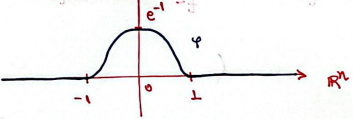
\includegraphics[height=0.5\textheight, width=0.5\textwidth, keepaspectratio]{./Images/bell_curve_05.png}
	\end{center}
	\caption{ilustração do gráfico da \(\alpha \) acima.}
\end{figure}

Seguiremos algumas etapas para realizar a confirmação dessa função.

\textbf{\underline{Primeira Etapa}:} mostrar que a função \(f:\mathbb{R}\rightarrow \mathbb{R}\) dada por
\[
	f(t) = \left\{\begin{array}{ll}
		e^{-\frac{1}{t}}, & \quad t> 0    \\
		0,                & \quad t\leq 0
	\end{array}\right.
\]
é \(\mathcal{C}^{\infty}\).
\begin{figure}[H]
	\begin{center}
		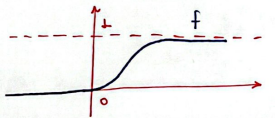
\includegraphics[height=0.5\textheight, width=0.5\textwidth, keepaspectratio]{./Images/plot_f_05.png}
	\end{center}
\end{figure}

Para isso, fica claro que o problema reside em derivar f no ponto \(t=0\), já que fora dele já é esperado que a f seja \(\mathcal{C}^{\infty}.\)

Começando pela continuidade, lembremos que, para todo s real ou complexo, temos
\[
	e^{s}=\sum\limits_{n=0}^{\infty}\frac{s^{n}}{n!} = 1+s+\frac{s^{2}}{2}+\frac{s^{3}}{3!}+\dotsc +\frac{s^{n}}{n!}+\dotsc ,
\]
donde segue que, para quaisquer s positivo e n natural,
\[
	e^{s}>\frac{s^{n}}{n!} \Rightarrow 0<e^{-s}<\frac{n!}{s^{n}}.
\]
Desta forma, tomando \(s=1/t\) para t positivo, obtemos
\[
	\lim_{t\to 0^{+}}e^{-\frac{1}{t}}\leq n!\lim_{t\to 0^{+}}t^{n}=0,
\]
mostrando a continuidade em \(t_{0}=0.\)

Agora, note que \(f'\equiv 0\) em \((-\infty, 0)\) e, se t for positivo,
\[
	f'(t)=(e^{-1/t})' = \frac{1}{t^{2}}e^{-\frac{1}{t}} = \frac{1}{t^{2}}f(t).
\]
No ponto \(t_{0}=0\), vemos que
\[
	\frac{f(t)-f(0)}{t} = \frac{e^{-\frac{1}{t}}}{t}
\]
e, fazendo \(n = 2\) em
\[
	e^{s}>\frac{s^{n}}{n!} \Rightarrow 0<e^{-s}<\frac{n!}{s^{n}},
\]
segue que o termo para t positivo da f satisfaz
\[
	f_{+}'(0)= 0,
\]
mostrando que f' é derivável em \(t_{0}= 0.\) Pela mesma estimativa, mas com \(n=3\), vemos que
\[
	0<\frac{e^{-\frac{1}{t}}}{t^{2}} < 3!t,
\]
donde obtemos
\[
	\lim_{t\to 0^{+}}f'(t)=0=f'(0),
\]
provando a continuidade de \(f'\).

A fim de fazer a indução, note que, para \(t > 0\),
\[
	f''(t)=-\frac{2}{t^{3}}e^{-\frac{1}{t}}+\frac{1}{t^{2}}f'(t)=-\frac{1}{t^{3}}f(t)+\frac{1}{t^{4}}f(t)=\biggl(\frac{1}{t^{4}}-\frac{2}{t^{3}}\biggr)f(t).
\]
Quando t e positivo e temos um natural n qualquer, isto nos dá a estimativa
\[
	0<\frac{1}{t^{n}}f(t)<(n+1)!t
\]
ou, mais geralmente ainda, se tivermos n e m dois naturais,
\[
	0<\frac{1}{t^{n}}f(t)<(m+n)!t^{m}.
\]
Daí, para todo n natural,
\[
	\lim_{t\to 0^{+}}\frac{1}{t^{n}}f(t)=0,
\]
sendo que o limite à esquerda já é obviamente 0. Consequentemente, para todo natural n,
\[
	\lim_{t\to 0}\frac{1}{t^{n}}f(t)=0,
\]
ou seja, se \(p:\mathbb{R}\rightarrow \mathbb{R}\) é qualquer polinômio, garantimos que
\[
	\lim_{t\to 0}p \biggl(\frac{1}{t}\biggr)f(t)=0.
\]

Agora, note que, dados t positivo e n natural,
\[
	f^{(n)}(t)=p_{n}\biggl(\frac{1}{t}\biggr)f(t)
\]
para algum polinômio \(p_{n}\) de grau 2n, enquanto que, para t negativo e natural,
\[
	f^{(n)}(t)=0.
\]
Sendo assim, para todo n natural,
\[
	\lim_{t\to 0}f^{(n)}(t)=0.
\]
Com isso, por indução e por um \hyperlink{tvm_cor}{\textit{corolário do TVM}}, podemos concluir que \(f^{(n)}(0)\) existe para todo n natural.

\begin{tcolorbox}[
		skin=enhanced,
		title=Lembrete!,
		after title={\hfill Corolário do TVM},
		fonttitle=\bfseries,
		sharp corners=downhill,
		colframe=black,
		colbacktitle=yellow!75!white,
		colback=yellow!30,
		colbacklower=black,
		coltitle=black,
		%drop fuzzy shadow,
		drop large lifted shadow
	]
	\hypertarget{tvm_cor}{
		\begin{crl*}
			Se \(g:[a, b]\rightarrow \mathbb{R}\) é contínua, derivável em \((a, b)\) e existe o limite
			\[
				\lim_{x\to a^{+}}g'(x)=L\in \mathbb{R},
			\]
			então g é derivável em a com
			\[
				g_{+}'(a)=L.
			\]
		\end{crl*}
	}
\end{tcolorbox}


\subsection{Aplicações Lineares Entre TVS's}
Dados dois TVS's \((E, \tau_{E})\) e \((F, \tau_{F})\), vamos analisar um pouco o que significa uma aplicação \(f:E\rightarrow F\) ser contínua. Quando ela for uma aplicação qualquer, dizer que f é contínua num ponto x de E significa que
\[
	(\forall U\in \tau_{F}:\; f(x)\in U,\; \exists V\in \tau_{E}:\; x\in V):\; f(V)\subseteq U,
\]
que equivale a
\[
	(\forall U\in \tau_{F}:\;0\in U,\; \exists V\in \tau_{E}:\;0\in V):\; y-x\in V \Rightarrow f(y)-f(x)\in U.
\]
Em particular, quando f é linear, a condição acima significa que para todo aberto de F contendo a origem, existe um aberto de E também contendo a origem tal que
\[
	y-x\in V \Rightarrow f(y-x)\in U,
\]
mostrando que, de certa forma, a continuidade de uma aplicação linear é ``uniforme'', e que vale o
\begin{theorem*}
	Seja \(f:E\rightarrow F\) linear entre TVS's. Então, f é contínua se, e somente se, f é contínua na origem.
\end{theorem*}
Este fato ganha uma nova visão quando as topologias dos TVS's vêm de seminormas:
\begin{prop*}
	Sejam \((E, \{p_{\alpha }\}_{\alpha \in L})\) e \((F, \{q_{\beta }\}_{\beta \in B})\) TVS's com topologias induzidas pelas normas e \(T:E\rightarrow F\) uma aplicação linear. São equivalentes:
	\begin{itemize}
		\item[i)] T é contínua; e
		\item[ii)] Para todo \(\beta \) na família de índices B, existem c positivo e índices \(\alpha_1, \alpha_2,\dotsc , \alpha_{n}\) de L tais que
		      \[
			      x\in E \Rightarrow q_{\beta }(Tx)\leq c \sum\limits_{j=1}^{n}p_{\alpha_{j}}(x),
		      \]
		      onde tanto c quanto os índices dependem apenas de T e de \(\beta\), não do x.
	\end{itemize}
\end{prop*}
\begin{proof*}
	Que (ii) implica em (i) fica claro a partir da definição das bases das topologias de E e F: dada uma semibola \(B_{\beta }(0; \varepsilon )\), segue que
	\[
		B=\bigcap_{j=1}^{n}B_{\alpha_{j}}\biggl(0; \frac{\varepsilon }{nc}\biggr)
	\]
	cumpre a condição \(T(B)\subseteq B_{\beta }(0; \varepsilon )\).

	Reciprocamente, se T é contínua em \(x_{0}=0\), então dado \(\beta \) em B e \(\varepsilon =1\), existe um aberto V de E com
	\[
		0\in V \quad\&\quad B_{\beta }(0; 1);
	\]
	logo, existe um aberto básico de E,
	\[
		B=\bigcap_{j=1}^{n}B_{\alpha_{j}}(0; \delta ),\quad \delta >0,
	\]
	com \(T(B)\subseteq T(V)\subseteq B_{\beta }(0;1).\) Com isso, dado um ponto x de E, temos dois casos a considerar:

	\textbf{\underline{Caso 1}:} quando \(\sum\limits_{j=1}^{n}p_{\alpha_{j}}(x)>0\). Neste caso, o valor
	\[
		\frac{\delta }{4 \sum\limits_{j=1}^{n}p_{\alpha_{j}}(x)}\in B,
	\]
	pois, para \(k=1,\dotsc ,n\), temos
	\[
		\frac{\delta }{2\sum\limits_{j=1}^{n}p_{\alpha_{j}}} p_{\alpha_{k}}(x)<\frac{\delta }{2},
	\]
	pois \(p_{\alpha_{k}}(x)\) em si é uma das parcelas do denominador; consequentemente,
	\[
		\frac{\delta }{2\sum\limits_{j=1}^{n}p_{\alpha_{j}}(x)} q_{\beta}(Tx)<1,
	\]
	mostrando que (ii) é válido neste caso ao tomarmos \(c=2/\delta >0.\)
	\begin{figure}[H]
		\begin{center}
			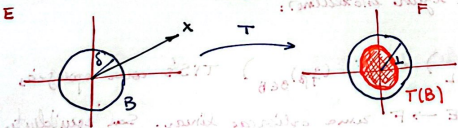
\includegraphics[height=0.5\textheight, width=0.5\textwidth, keepaspectratio]{./Images/application_05.png}
		\end{center}
		\caption{após aplicar T, a limitação por um fator de \(\delta \) torna-se limitação por 1.}
	\end{figure}

	\textbf{\underline{Caso 2}:} quando \(\sum\limits_{j=1}^{n}p_{\alpha_{j}}(x)=0.\) Aqui, para todo t real, segue que \(tx\) pertence a B, pois
	\[
		p_{\alpha_{j}}(tx)=|t|p_{\alpha_{j}}(x)=0, \quad \forall t\in \mathbb{R},
	\]
	donde temos \(T(tx)\in B_{\beta }(0; 1)\), isto é,
	\[
		tq_{\beta }(Tx)<1,\quad \forall t\in \mathbb{R},
	\]
	implicando que \(q_{\beta }(Tx)=0\), portanto, (ii) vale com a mesma constante. \qedsymbol
\end{proof*}

\begin{tcolorbox}[
		skin=enhanced,
		title=Observação,
		fonttitle=\bfseries,
		colframe=black,
		colbacktitle=cyan!75!white,
		colback=cyan!15,
		colbacklower=black,
		coltitle=black,
		drop fuzzy shadow,
		%drop large lifted shadow
	]
	O caso que mais nos interessa, a princípio, é aquele em que \(F=\mathbb{C}\), já que a proposição acima fornecerá, então, em termos de estimativa, uma caracterização da continuidade dos funcionais lineares \(u:E\rightarrow \mathbb{C}\) em E.
\end{tcolorbox}

\begin{crl*}
	Seja \(u:E\rightarrow \mathbb{C}\) um linear no TVS \((E, \tau )\) com a topologia dada por uma família de seminormas \(\{p_{\alpha }\}_{\alpha\in L}.\) Então, u é contínua se, e somente se, existem \(\alpha_{1},\dotsc , \alpha_{n}\) em L e c positivo tais que
	\[
		x\in E \Rightarrow |\left< u, x \right>|\leq c\sum\limits_{j=1}^{n}p_{\alpha_{j}}(x).
	\]
\end{crl*}
\begin{proof*}
	A topologia do TVS \(\mathbb{C}\) provém de uma única norma, \(|\cdot |\). Portanto, só há uma escolha para o \(\beta \in B\) na proposição anterior. \qedsymbol
\end{proof*}

\begin{example}[Funcionais de \(\mathcal{C}(\Omega )\) em \(\mathbb{C}\).]
	Um funcional \(u:\mathcal{C}(\Omega )\rightarrow \mathbb{C}\) linear é contínuo se, e somente se, existem um compacto \(K\) contido em \(\Omega \) e \(c > 0\) tais que
	\[
		|\left< u, \varphi  \right>|\leq c \sup_{x\in K}|\varphi(x)|, \quad \varphi \in \mathcal{C}(\Omega ),
	\]
	pois as seminormas de \(\mathcal{C}(\Omega )\) são
	\[
		p_{j}(\varphi )=\sup_{x\in K_{j}}|\varphi(x)|.
	\]
	Em particular, u tem suporte compacto:
	\[
		\mathrm{supp}(\varphi )\cap K= 0 \Rightarrow \left< u, \varphi  \right>=0.
	\]

	Este funcionais podem ser usados, ou definirem, as medidas booleanas (pode estar errado) em \(\Omega \) (c.f. Folland, pags. 212 e 213).
\end{example}
\begin{example}[Espaço das Distribuições com Suporte Compacto]
	Um funcional \(u:\mathcal{C}^{\infty}(\Omega )\rightarrow \mathbb{C}\) é linear e contínuo se, e somente se, existem um compacto K, uma constante positiva c e \(m\in \mathbb{N}\cup \{0\}\) tal que
	\[
		|\left< u, \varphi  \right>| \leq c \sum\limits_{|\alpha |\leq m}^{}\sup_{x\in K}|\partial^{\alpha }\varphi (x)|,
	\]
	pois as seminormas de \(\mathcal{C}^{\infty}(\Omega )\) são
	\[
		p_{(m, j)}(\varphi ) = \sum\limits_{|\alpha |\leq m}^{} \sup_{x\in K_{j}}|\partial ^{\alpha }\varphi(x)|,
	\]
	onde a estimativa ocorre tomando o maior m e o maior j da soma em (ii), tendo em vista que
	\[
		p_{(m, j)}(\varphi )\leq p_{(m+1, j)}(\varphi )\quad\&\quad p_{(m, j)}(\varphi )\leq p_{(m, j+1)}(\varphi ).
	\]

	Como antes, vale que u ter suporte compacto é como se fosse \(u=0\) em \(\Omega \setminus{K}\), então
	\[
		\mathrm{supp}(\varphi )\cap K=\emptyset \Rightarrow \left< u, \varphi  \right>=0.
	\]
	Note também que o m, ou seja, a ordem da derivada que aparece na estimativa, depende do u e não das \(\varphi \)'s, o que significa que apenas as derivadas até a ordem m influenciam na continuidade de u.
\end{example}
\begin{def*}
	Um tal u do exemplo acima é o que chamamos de \textbf{distribuição de suporte compacto}, e o espaço das \textbf{distribuições de suporte compacto} em \(\Omega \), \(\mathcal{E}'(\Omega )\), é o espaço dual de \(\mathcal{C}^{\infty}(\Omega )\), ou seja,
	\[
		\mathcal{E}'(\Omega )=[\mathcal{C}^{\infty}(\Omega )]'. \quad \square
	\]
\end{def*}

\begin{example}[Espaço das Distribuições Temperadas]
	Um funcional \(u:\mathcal{S}(\mathbb{R}^{n})\rightarrow \mathbb{C}\) linear é contínuo se, e somente se, existem c positivo e \(m, n\in \mathbb{N}\cup \{0\}\) tais que
	\[
		|\left< u, \varphi  \right>|\leq c \sum\limits_{|\alpha |\leq m}^{} \sup_{}(1+|x|)^{N}|\partial^{\alpha }\varphi (x)|, \quad \forall \varphi \in \mathcal{S},
	\]
	pois, para todos \(\varphi,\) N e \(\alpha \),
	\[
		\Vert \varphi  \Vert_{(N, \alpha )}\leq \Vert \varphi  \Vert_{(N+1, \alpha )},
	\]
	então pegamos o maior N e, do número finito \(\alpha_1, \alpha_2,\dotsc ,\alpha_{n}\in \mathbb{Z}_{+}^{n}\), tomamos \(m = \max\limits_{j=1,\dotsc , p }|\alpha_{j}|\) na estimativa (ii) da proposição.
\end{example}
\begin{def*}
	Um u do exemplo acima é o que chamamos de \textbf{distribuição temperada}, e o espaço das \textbf{distribuições temperadas}, \(\mathcal{S}'(\mathbb{R}^{n} )\), é o espaço dual de \(\mathcal{S}(\mathbb{R}^{n} )\), ou seja,
	\[
		\mathcal{S}'(\mathbb{R}^{n} )=[\mathcal{S}(\mathbb{R}^{n} )]'. \quad \square
	\]
\end{def*}

\subsection{Dual de Espaços Vetoriais Topológicos: topologia fraca-*}
Seja \((E, \tau )\) um TVS, e indiquemos por E' o seu espaço \textbf{dual topológico} (distinto do dual algébrico \(E^{*}=\{u:E\rightarrow \mathbb{C}:\; u\text{ é linear}\}\)), que consiste de \textbf{todos os funcionais lineares contínuos em E}, onde consideramos \(\mathbb{C}\) munido de sua topologia usual.

Nosso objetivo é munir E' com uma topologia localmente convexa e Hausdorff; sempre que o considerarmos assim, a topologia usada será a \textbf{topologia fraca-*}, ou seja, a definida pelas seminormas
\begin{align*}
	p_{x}: & E'\rightarrow \mathbb{C}                           \\
	       & u\mapsto p_{x}(u) \coloneqq |\left< u, x \right>|.
\end{align*}
Note que esta topologia é a induzida de \(\mathcal{F}(E; \mathbb{C})\supseteq E'\), de modo que \(u_{n}\substack{* \\ \longrightarrow \\ }u\), ou \(u_{n}\substack{E' \\ \longrightarrow \\ }u\), quando \(\{u_{n}\}\) convergir pontualmente para u em E, ou seja,
\[
	p_{x}(u_{n}-u)\substack{ \\ \longrightarrow \\ n\to \infty}0,\; \forall x\in E \Longleftrightarrow |\left< u_{n}, x \right>-\left< u, x \right>|\substack{ \\ \longrightarrow \\ n\to \infty}0,\; \forall x\in E.
\]
O fato desta topologia ser Hausdorff se dá pois \(\{p_{x}\}_{x\in E}\) é separante. Diferentemente do que ocorre com o dual de um espaço normado, que é sempre completo, não podemos dizer o mesmo de um TVS qualquer: a resposta dependerá da topologia \(\tau \) de E. Quando E é um espaço de Fréchet, por exemplo, é verdade que seu dual é completo devido ao teorema de Banach-Steinhauss, mas isto é assunto para o futuro.

\end{document}
